% vim:autoindent:set textwidth=78:

\section{Map Composer}\label{label_mapcomposer}

The map composer is a feature that provides limited layout and printing
capabilities. The composer allows you to add elements such as the QGIS map
canvas, legend, scalebar, images, and text. You can size and position each item and
adjust the properties to create your layout. The result can be printed,
exported as an image, or exported to SVG.

To access the map composer, click on the \toolbtntwo{mActionFilePrint}{Print}
button in the toolbar or choose \mainmenuopt{File} > \dropmenuopttwo{mActionFilePrint}{Print}.

\subsection{Using Map Composer}\label{label_usemapcomposer} 

To use the map composer, first add the layers you
want to print to QGIS. The layers should be rendered and symbolized to your
liking prior to composing the map. 

\begin{figure}[ht]
   \begin{center}
   \caption{Map Composer}\label{fig:map_composer_blank}\smallskip
   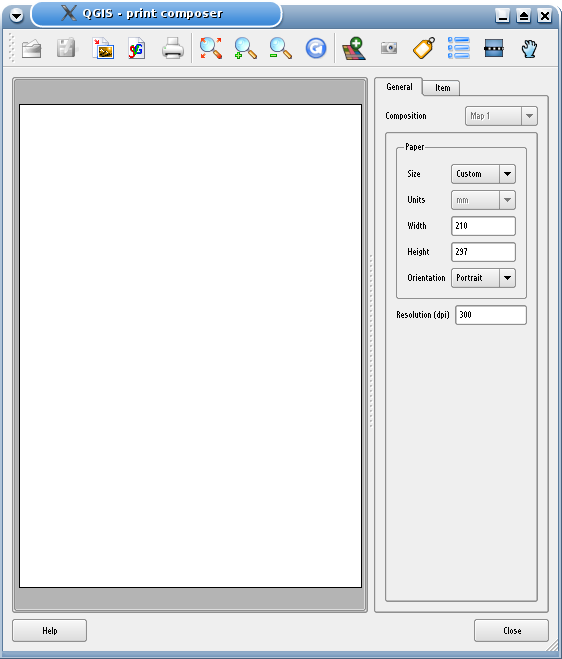
\includegraphics[clip=true, width=14cm]{map_composer_blank09}
\end{center}  
\end{figure}

Opening the map composer provides you with a blank canvas to which you can add
the current map view, legend, scalebar, and text. Figure
\ref{fig:map_composer_blank} shows the initial view of the map composer before
any elements are added.

The map composer has two tabs: \tab{General} and \tab{Item}. The General tab
allows you to set the paper size, orientation, and resolution for the map.
The Item tab displays the properties for the currently selected map element.
By selecting an element on the map (eg. legend, scalebar, text, etc.) and
clicking on the \tab{Item} tab, you can customize the settings.

You can add multiple elements to the composer. This allows you to have more
than one map view and legend in the composer. Each element has its own
properties and in the case of the map, its own extent.

\subsubsection{Adding a Map to the Composer}

To add the QGIS map canvas to the map composer, click on the
\toolbtntwo{composer_add_image}{Add a new map} button in toolbar. Drag a rectangle on the composer canvas to add the
map. You can resize the map later by clicking on the \button{Select/move item}
button, clicking on the map, and dragging one of the handles in the corner of
the map. With the map selected, you can also resize the map by specifying the
width and height on the Item properties tab.

The map is linked to the QGIS map canvas. If you change the view on the map
canvas by zooming or panning, you can update the map composer view by
selecting the map in composer and clicking on the \button{Set Extent} button.
You can also change the composer view by specifying a map scale. To set the
view to a specific scale:

\begin{enumerate}
\item Choose \selectstring{Set}{Scale (calculate extent)}
\item Enter the scale denominator in the scale box
\item Press Enter
\end{enumerate} 

\subsubsection{Adding other Elements to the Composer} 
 
Already existing QGIS templates can be used to easily load and adapt map
layouts. To open an existing template, click on the
\toolbtntwo{composer_open_template}{Open Template} button. Choose a template and
customize its appearance. 

To add a logo, north arrow or any  kind of image to the composer, click on
the \toolbtntwo{composer_add_image}{Add Image} button. The image will 
be placed on the composer canvas and you can move it where you like. 

A legend can be added to the composer canvas and customized to show only the
desired layers. To add a legend, click on the
\toolbtntwo{composer_add_legend08}{Add Vector Legend} button. The legend will be
placed on the composer canvas and you can move it where you like. Click on
the \tab{Items} tab to customize the appearance of the legend, including
which layers are shown.

To add a scalebar to the composer, click on the
\toolbtntwo{composer_add_scalebar08}{Add Scalebar} button. Use the \tab{Item}
tab to customize the segment size, number of segments, scalebar units, size,
and font for the scalebar.

You can add text labels to the composer by clicking on the
\toolbtntwo{composer_add_label}{Add New Label} button. Use the \tab{Item} tab
while the text is selected to customize the settings or change the default text.

Figure \ref{fig:map_composer_complete} shows the map composer after adding
each type of map element.
\begin{figure}[h]
   \begin{center}
   \caption{Map Composer with map view, legend, scalebar, and text added}\label{fig:map_composer_complete}\smallskip
   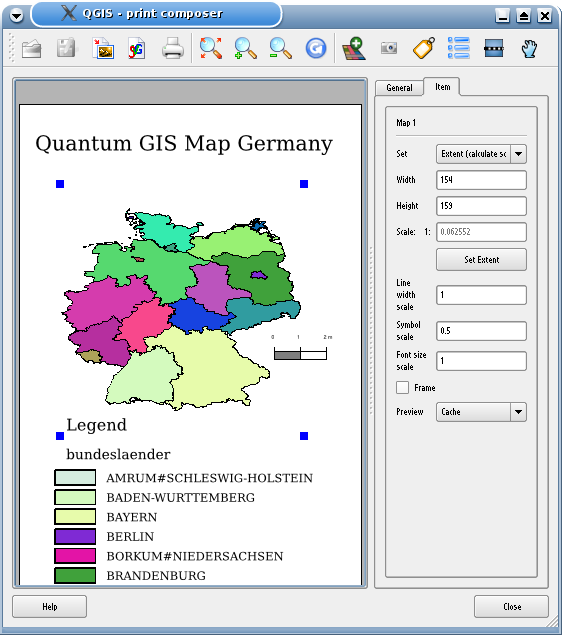
\includegraphics[clip=true, width=14cm]{map_composer09}
\end{center}  
\end{figure}

\subsubsection{Other Features}

The map composer has navigation tools to zoom in and out. To zoom in, click
the \button{Zoom in} tool. The map composer canvas will be scaled by a factor to 2. Use
the scrollbars to adjust the view to the area of interest. Zooming out works
in a similar fashion.

If you find the view in an inconsistent state, you can use the \button{Refresh} button
to redraw the map composer canvas.

\subsubsection{Creating Output}

The map composer allows you to print the map to a printer, export to a PNG or
export to SVG. Each of these functions is available from the composer toolbar.

To save the composer canvas as a templates, click on the
\toolbtntwo{composer_save_template}{Save Template As} button. Browse to the directory 
you like and save a template to use it again for another map canvas.

It is possible to export the result as an image by clicking on the
\toolbtntwo{composer_export_image}{Export as image} button. 

To export the composer canvas as an  SVG (Scalable Vector Graphic), click on
the \toolbtntwo{composer_export_svg}{Export as SVG} button. \textbf{Note:}
Currently the SVG output is very basic. This is not a QGIS problem, but a
problem of the underlaying Qt library. This will be sorted out in future versions.
 
